\subsection{The Query Model}\label{section:queryModel}

\subsubsection*{Continuous Query Model}

In the context of our application, taking into account that the input data of our system takes the form of a continuous data stream, 
we categorize our query model under the \emph{continuous query} model \cite{CQ-babu2001continuous, CQ-zaniolo2012logical}. 
The continuous query model is the ideal query model for applications considering queries evaluated over data streams (unbounded sequences of timestamped data items), 
in contrast with classical query evaluation processes, where the data to query is stable, with few or infrequent updates. 
Although, part of the data source of our application is stable (the stable bank database), the input of our system consists of a data stream, 
data in motion and continuously changing, as it is the ATM transactions input data stream.\\ 

In our work, we tackled the problem of evaluating continuous queries corresponding to anomalous patterns of ATM transactions 
against a continuously evolving property graph, PG, representing a bank database. 
The bank database is continuously evolving due to the input ATM transactions data stream that it receives continuously. 
The anomalous patterns of ATM transactions are identified in the volatile (PG) subgraph of the considered database. 
With this, a query on our PG database can be defined as a PG graph pattern with constraints over some of its properties. 
Evaluating such a query consists on identify if there is a subgraph of the database that matches the given graph pattern and satisfies its constraints.

\iffalse
\subsubsection*{Fraud Patterns Definition}

It is not trivial to establish what is and in which circumstances an ATM transaction can be considered anomalous. Based on a work that have addressed this characterization \cite{FP-magdalena2021artificial} we intend to find a proper characterization and then define the graph patterns associated to these anomalies. The exact topology of an anomaly will depend on its own nature. Moreover, definition of patterns can be beyond ATM transactions by considering online card transactions. In what follows, we propose a characterization of some possible anomalous patterns of ATM transactions and the definition of their associated PG graph patterns. 

\begin{enumerate}
\renewcommand{\labelenumi}{\Roman{enumi}.} % Roman numerals for the list
    \item Card cloning characterization
    \item Lost-and-stolen card characterization
    %\item Anomalous amount of withdrawals in a time period
    \item Other possible fraud scenarios
\end{enumerate}


\paragraph{I - Card Cloning Characterization\\\\}

\emph{Card cloning} can be defined as a "type of fraud in which information on a card used for a transaction is covertly and illegally duplicated. Basically, it’s a process thieves use to copy the information on a transaction card without stealing the physical card itself. This information is then copied onto a new or reformatted card, allowing criminals to use it to make fraudulent purchases or gain unauthorized access to a person’s accounts."\cite{FP-unit21_card_cloning}.\\

There are many possible ways to detect a card cloning scenario, among others, the analysis of the customer's transaction data to construct typical transaction behaviors so to be able to detect uncommon transaction behaviors. However, in our work we propose an alternative possible method based on a PG graph pattern detection.\\

The method consists on detecting abnormal card-ATM activity of the same card at different ATMs taking place within an unfeasible time distance difference. That is, when a transaction is made at an ATM, and after that, another transaction is initiated with the same card at a different ATM, such that the distance between the two is impossible to be covered within the time between the transactions.
The detection of this anomalous scenario is represented on the PG graph pattern of the Figure \ref{img:graphPattern-1}. 

\begin{figure}[H]
  \centering
  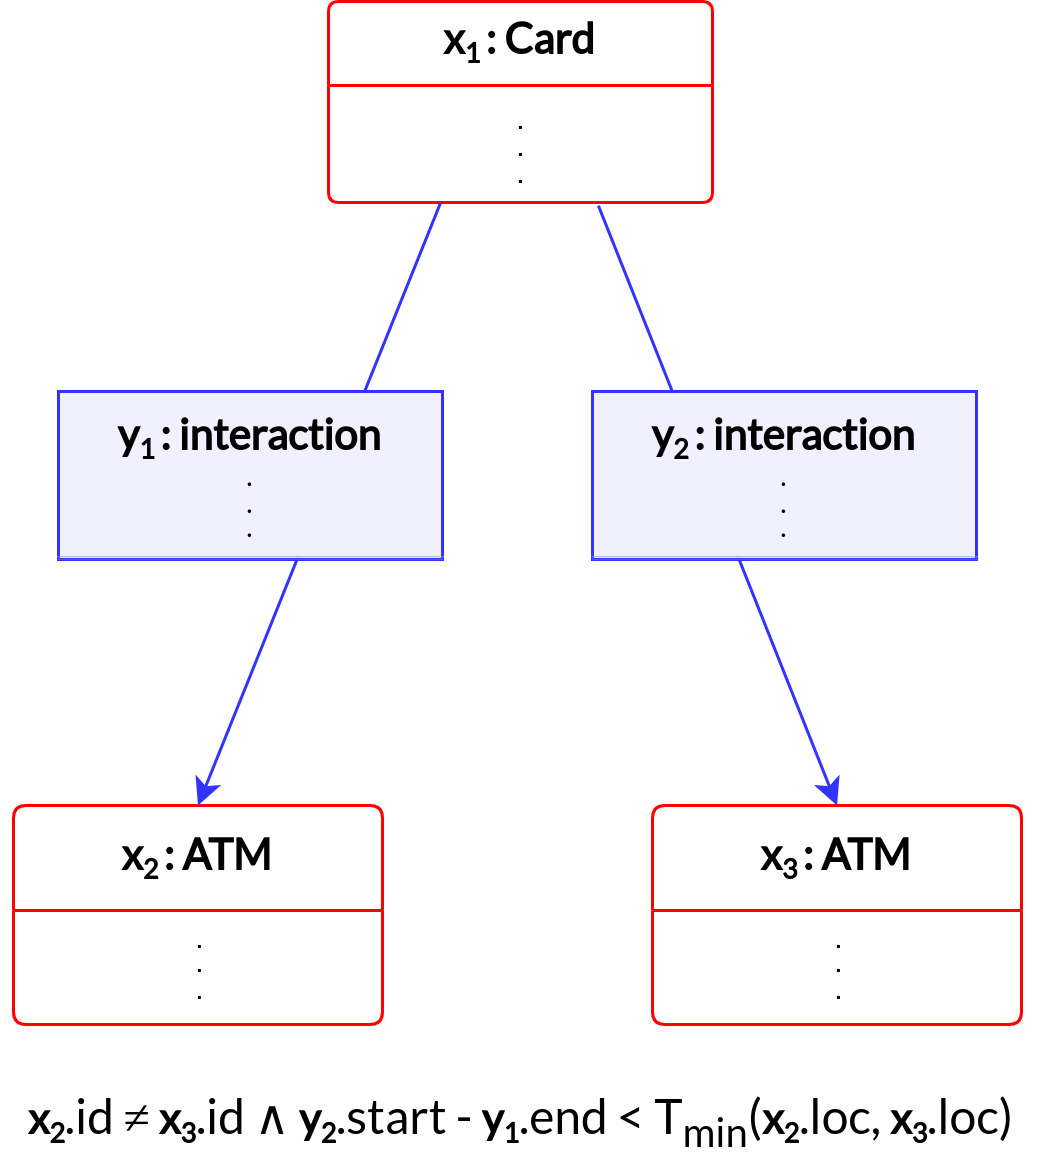
\includegraphics[scale = 0.8]{images/2-QueryModel/graphPattern-1.png}
  \caption{Property graph pattern - Card cloning characterization}
  \label{img:graphPattern-1}
\end{figure}

The pattern consists on a \texttt{Card} entity $x_1$, having two \texttt{interaction} relations $y_1$ and $y_2$ with two different \texttt{ATMs} $x_2$ and $x_3$, respectively, such that the time difference between the ending time of the first \texttt{interaction} $y_1.\textit{end}$ and the starting time of the second \texttt{interaction} $y_2.\textit{start}$, is not sufficient to cover the minimum time needed to travel from the first to the second \texttt{ATM} location $T_{min}(x_2.\textit{location}, x_3.\textit{location})$. As a whole:

$$
\small
x2.id \ne x3.id \ \land \ y_2.\textit{start} - y_1.\textit{end} < T_{min}(x_2.\textit{location}, x_3.\textit{location})
$$

where $x_2.\textit{location}$ location represents the location coordinates pair of the $x_2$ ATM: $x_2.location = (x_2.loc\_latitude, x_2.loc\_longitude)$. Same for the \texttt{ATM} $x_3$.\\

An example of this kind of anomalous card-ATM interaction, could be one as represented on Figure \ref{img:graphPattern-1-Example}, in which an ATM interaction with a certain card is finished at time 22:14 in Barcelona, and then another interaction with that same card starts at time 22:56 of that same day in Madrid. Clearly this should be reported as this kind of anomalous scenario since it is impossible, for the time being, to cover the distance between these two cities in that time difference.

\begin{figure}[H]
  \centering
  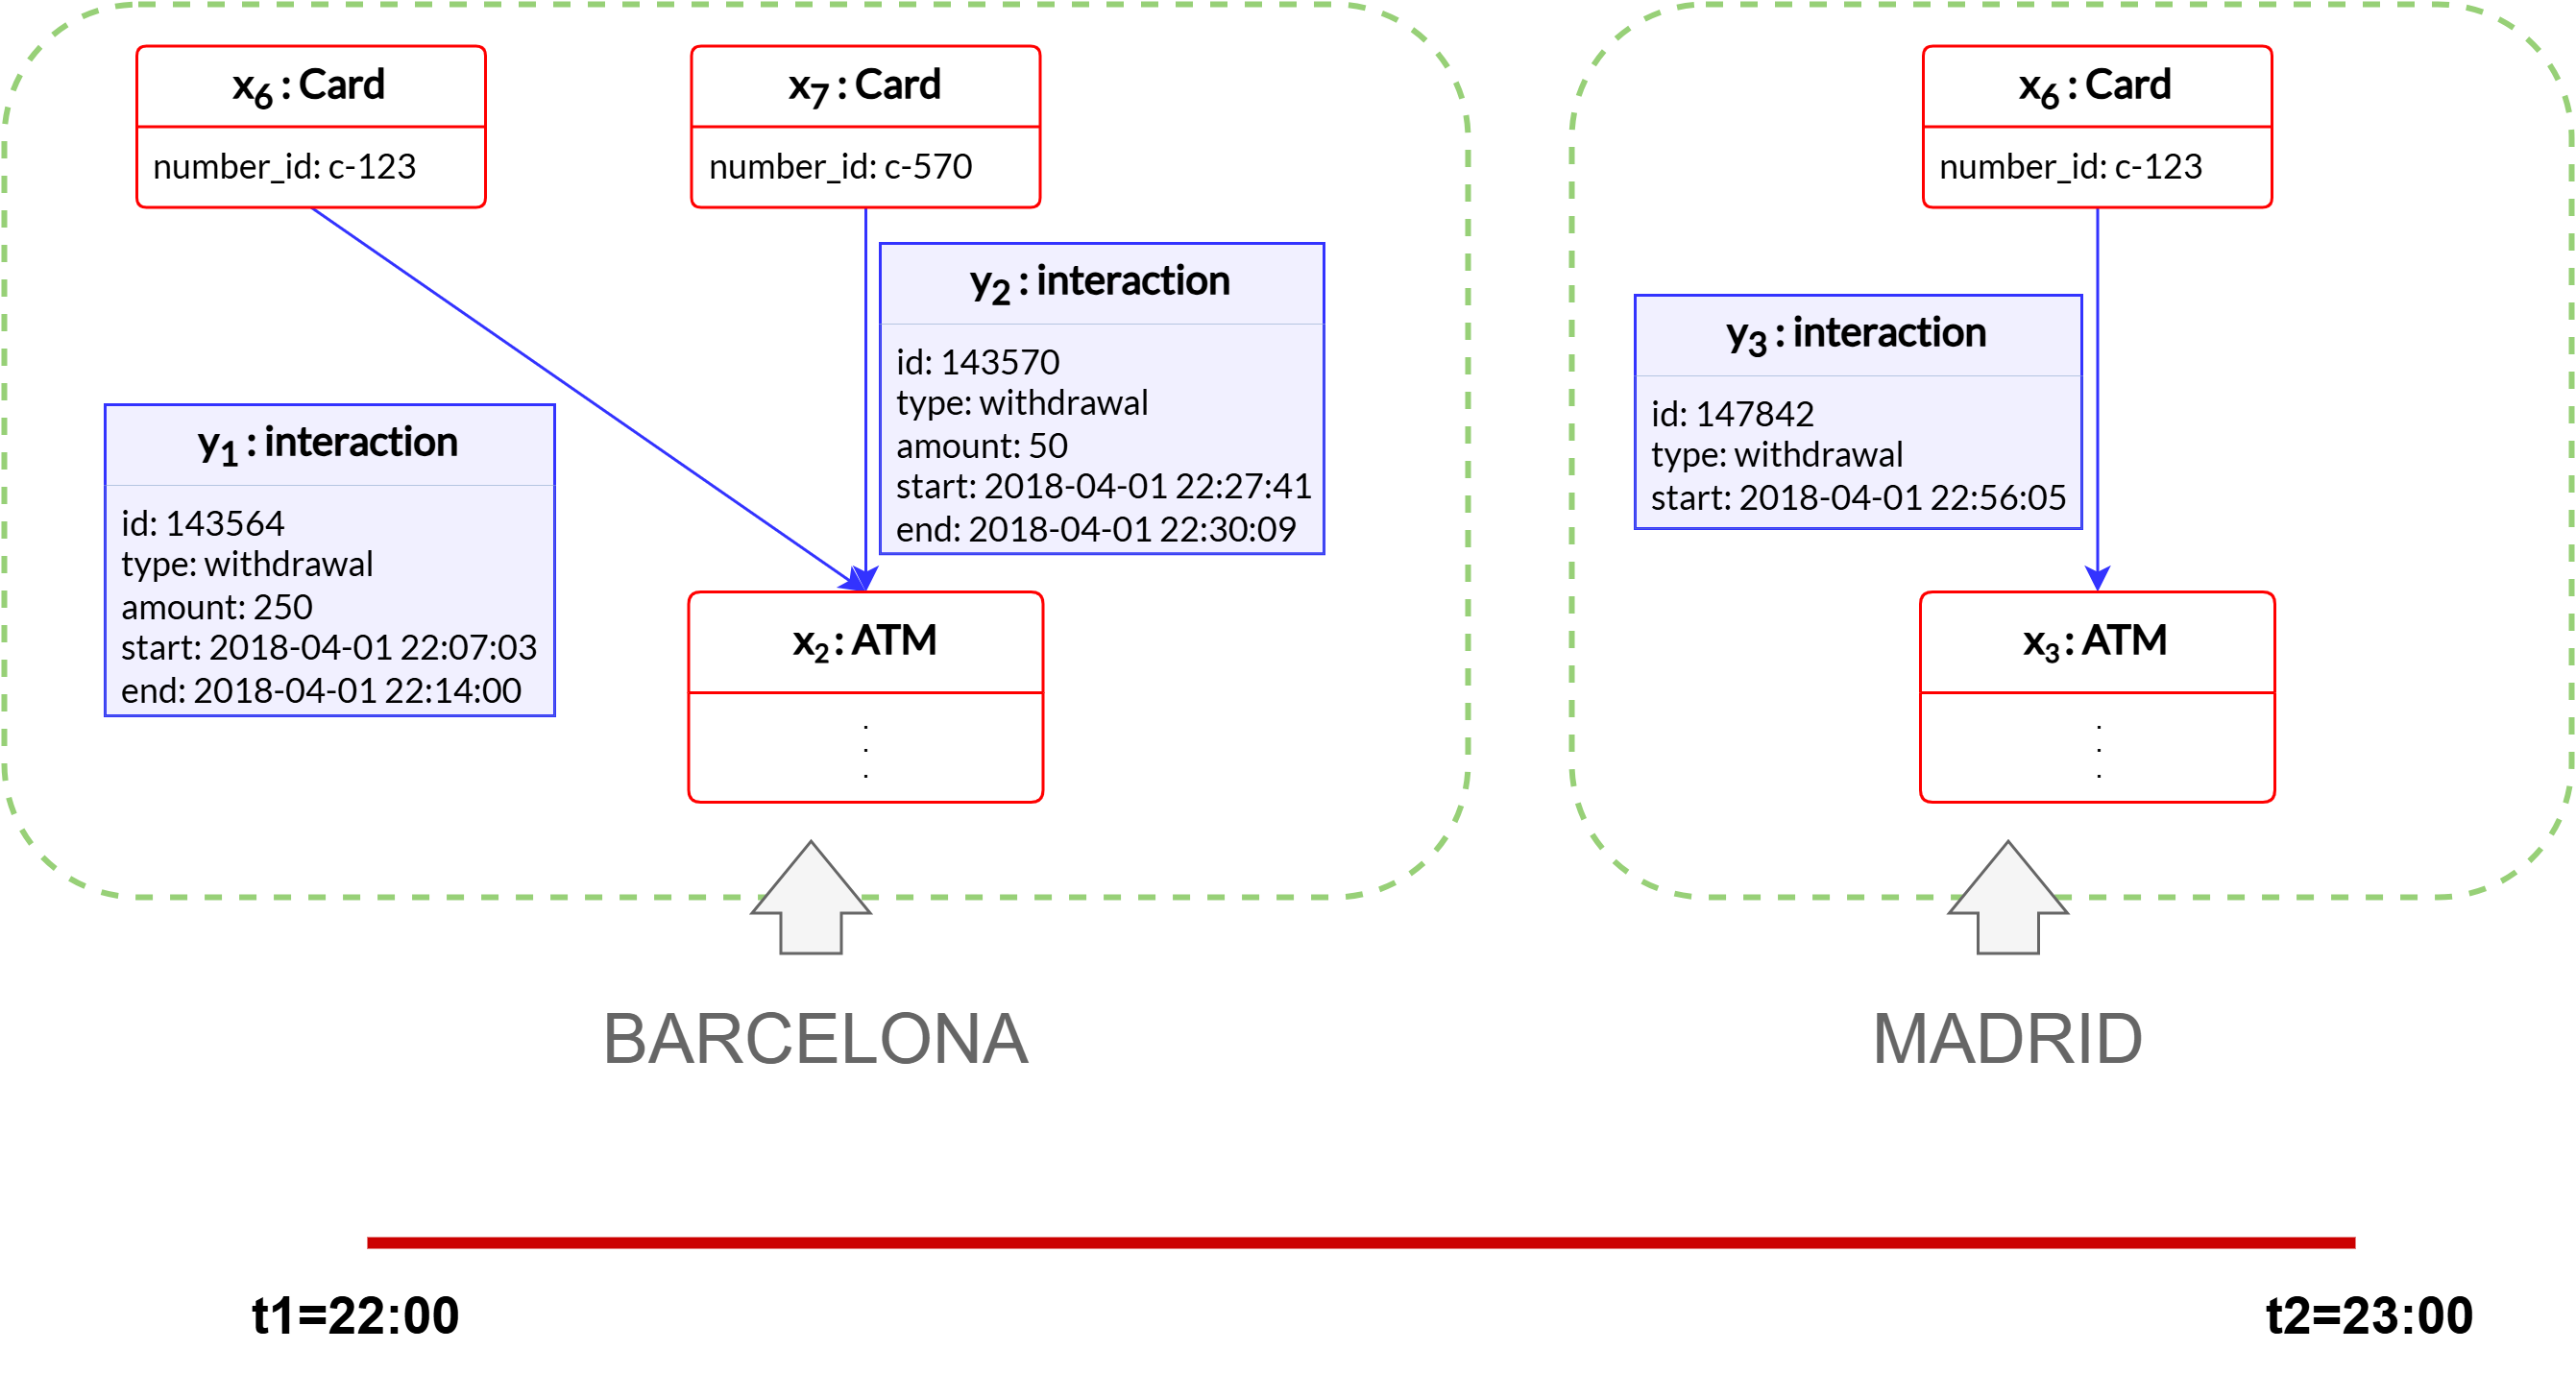
\includegraphics[scale = 0.7]{images/2-QueryModel/FP1-Example.png}
  \caption{Card cloning characterization - an example}
  \label{img:graphPattern-1-Example}
\end{figure}

\paragraph{II - Lost-and-Stolen Card Characterization\\\\}

"Lost-and-stolen card is the fraud scenario produced when a card is physically stolen or is lost, and is then used by a criminal, posing as you, to obtain goods and services" \cite{FP-lost-and-stolen-americanexpress2025}.\\

A possible way that we propose to detect this kind of fraud scenario is through the tracking of a typical behavior that it is produced when the card is used by the criminal. That is, when obtained, the fraudster tries to do as many as possible money withdrawals in different ATMs before the owner of the card realises and asks the bank to freeze the card. The detection of this kind of fraud scenario is modeled with a PG graph pattern as the one represented on Figure \ref{img:graphPattern-2}.

\begin{figure}[H]
  \centering
  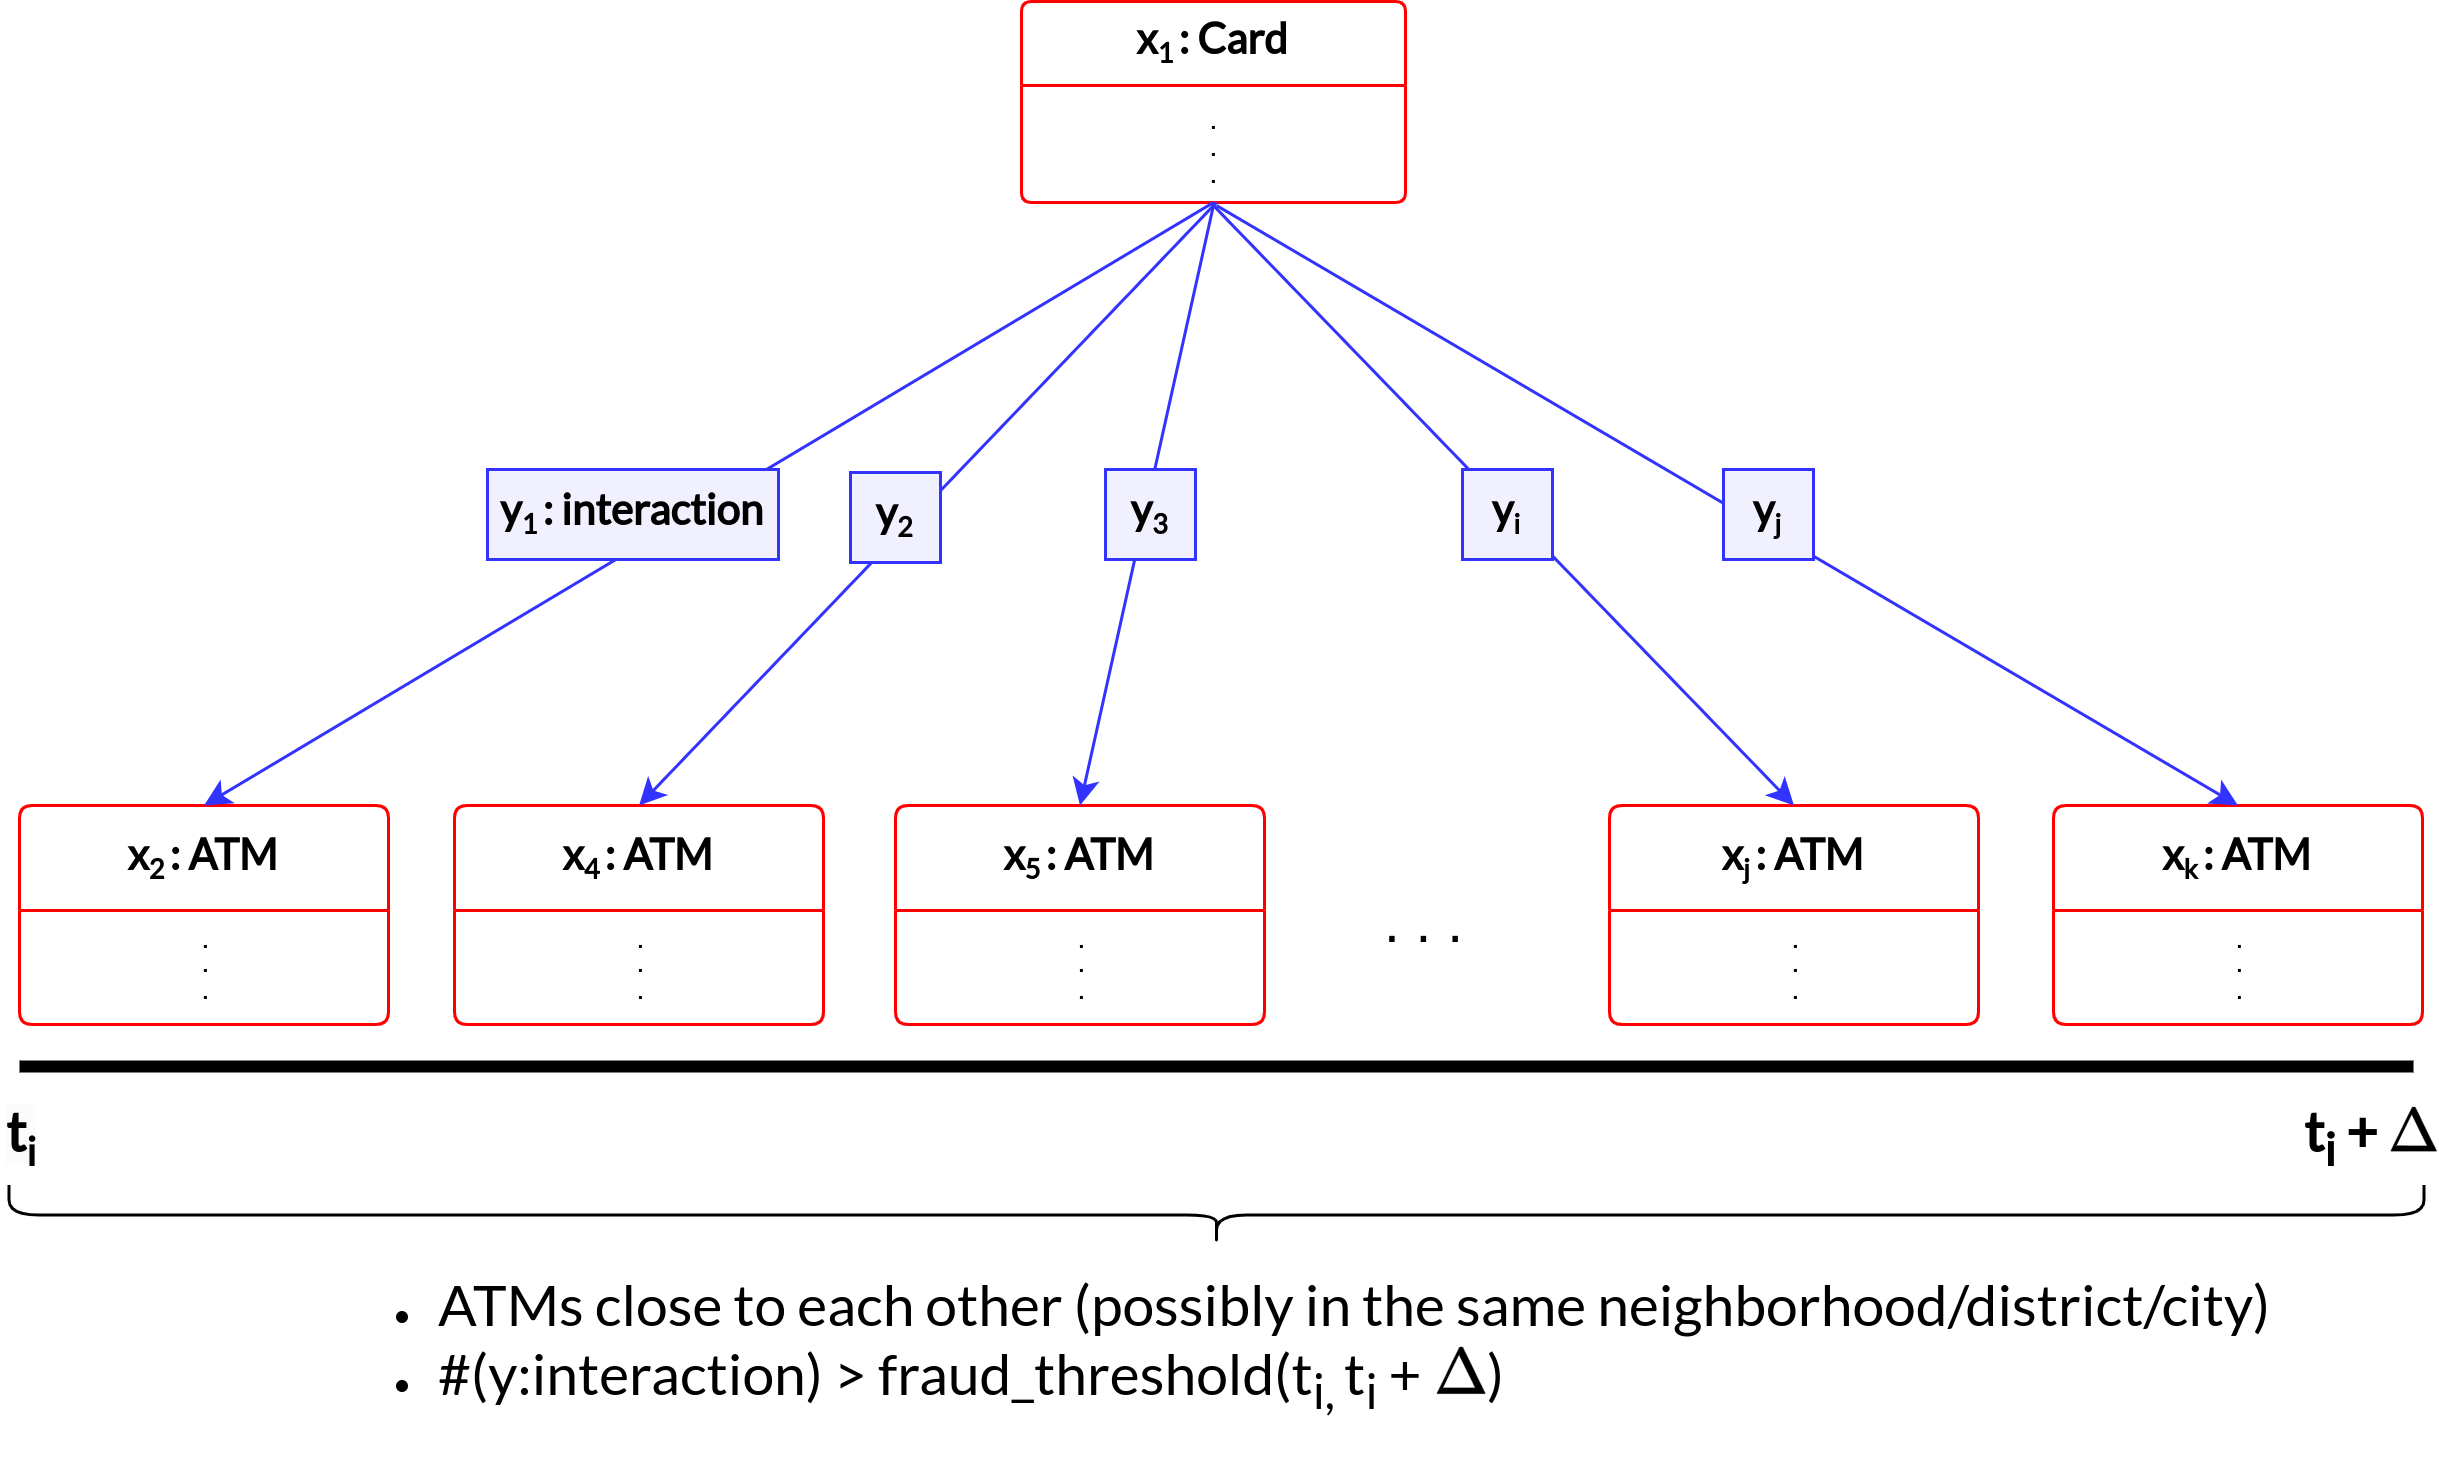
\includegraphics[scale = 0.7]{images/2-QueryModel/graphPattern-2.png}
  \caption{Property graph pattern - Lost-and-stolen card characterization. The interactions $y_1,...,y_j$ depicted are of the \emph{type} withdrawal}
  \label{img:graphPattern-2}
\end{figure}

On it we define a \texttt{Card} entity $x_1$ having a number $k$ of \texttt{interactions} $y$ at different \texttt{ATMs} $x_2 ... x_k$ within a time interval $[t_i, t_i + \Delta]$, where $t_i = y_1.\textit{start}$ and $t_i + \Delta = y_j.\textit{start}$, such that $k$ is considered to be an usual high number of withdrawals for that time interval. A reference for the usual number of withdrawals on a certain time interval for a specific cardholder can be obtained from the gathered cardholder behavior \emph{withdrawal\_day} \texttt{Card} entity property.
Another indicator of this scenario to be considered could also be the \emph{amount} value of the withdrawal operations performed, which, in these scenarios, is normally a low value to prevent that the card owner realises.

\paragraph{III - Other possible fraud scenarios\\\\}

Some other anomalous scenarios for which more graph patterns could be defined are:
\begin{itemize}
    \item \textbf{Anomalous location usage}: When a transaction is made in a location out of the threshold distance of the usual/registered address of the cardholder.
    \item \textbf{Anomalous number of operations}: Related with the II pattern characterized, we could also define a graph pattern related with a higher than average number of operations of any kind (withdrawal, inquiry, transfer or deposit) for a cardholder in a certain time interval.
    \item \textbf{Anomalous high expenses:} Similar to the II pattern, but in this case, not considering only the number of the withdrawal operations performed on a certain time interval, but the amount of the withdrawal operations on a certain time interval. This could indicate an anomalous behavior of the cardholder, withdrawing an amount of money way higher for a considered time interval.
\end{itemize}
\fi

\subsubsection*{Fraud Patterns Algorithmic Description}

So far, among all the characterized anomalous scenarios as PG graph patterns, for our proof of concept, 
we implemented the detection of the first defined fraud graph pattern, the fraud graph pattern I (defined in \ref{sub:anomalouspatterns}), 
related with the card cloning characterization.\\

A first attempt to detect fraud pattern I in our setting is to compare, for each new transaction of a given card, 
its initial time against the final time of all the previous transactions of the same card. 
This procedure is given in Algorithm \ref{alg:check-fraud-1}. 
Note that $\mathsf{S_c}$ refers to an individual node \texttt{Card} $\mathsf{c}$ subgraph of our volatile property graph. 
It stores all the card-ATM interactions $\mathsf{e_c}$ that are made with \texttt{Card} $\mathsf{c}$ for a considered time interval. 
$\mathsf{e_{new}}$ is the new incoming edge belonging to \texttt{Card} $\mathsf{c}$, such that it is an opening interaction edge. 
Note that this is this way since for the incoming closing interaction edges, we will not perform any fraud checking operation \text{CheckFraud()}.

\begin{algorithm}[H]
    \small
    \begin{algorithmic}[1]
    \REQUIRE $\mathsf{S_c}$ refers to an individual node \texttt{Card} $\mathsf{c}$ subgraph of our volatile property graph. 
    It stores all the card-ATM interactions $\mathsf{e_c}$ that are made with \texttt{Card} $\mathsf{c}$ for a considered time interval. 
    The interactions are stored sorted by time.
    \REQUIRE $\mathsf{e_{new}}$ is the new incoming edge belonging to \texttt{Card} $\mathsf{c}$
    \STATE $\texttt{fraudIndicator} \gets \texttt{False}$
    \STATE $i \gets |S_c|$
    \WHILE{$i > 0$ \AND \texttt{fraudIndicator} = \texttt{False}}
      \STATE $e_i \gets S_c[i]$
      \STATE $\texttt{t\_min} \gets \text{obtain\_t\_min}(e_i, e_{new})$
      \STATE $\texttt{t\_diff} \gets e_{new}.start - e_i.end$
      \IF{$\texttt{t\_diff} < \texttt{t\_min}$}   
        \STATE $\text{createAlert}(e_i, e_{new})$
        \STATE $\texttt{fraudIndicator} \gets \texttt{True}$
      \ENDIF
      \STATE $i \gets i - 1$
    \ENDWHILE
    \end{algorithmic}
    \caption{$\text{CheckFraud}(\mathsf{S_c}, \mathsf{e_{new}})$ -- \textbf{initial version}}
    \label{alg:check-fraud-1}
\end{algorithm}

There are some aspects and decisions of this algorithm that are worth to describe:

\begin{itemize}
    \item \textbf{Pairwise detection}. The checking of the anomalous fraud scenario is executed 
    by doing the check between the new incoming edge $\mathsf{e_{new}}$ and each of the edges $\mathsf{e_i}$ of the \texttt{Card} $\mathsf{c}$ subgraph $\mathsf{S_c}$.
    \item \textbf{Backwards order checking}. The pairs $(\mathsf{e_{new}, e_i})$ are checked in a backwards time traversal order of the edges of the $\mathsf{S_c}$ subgraph, starting with the most recent edge of the subgraph and ending with the oldest.  
    \item \textbf{Stop the checking whenever the first anomalous scenario is detected}. Whenever an anomalous scenario corresponding to a pair $(\mathsf{e_{new}, e_i})$ is detected 
    we stop the checking at this point and emit the corresponding alert. There is no need to continue the checking with previous edges of $\mathsf{S_c}$. 
    \item \textbf{Emission of the pair $(\mathsf{e_{new}, e_i})$ as the alert}. The alert is composed by the pair $(\mathsf{e_{new}, e_i})$ that is detected to cause the anomalous scenario. Both edges are emitted in the alert since we do not know which is the one that is the anomalous. On the one hand, it can be $\mathsf{e_i}$, which is previous to $\mathsf{e_{new}}$, in the case that $\mathsf{e_i}$ at the moment it arrived it did not cause any alert with the previous edges/transactions of the subgraph and it causes it now with a new incoming edge $\mathsf{e_{new}}$ which is a regular transaction of the client. On the other hand, it can be $\mathsf{e_{new}}$, which is the last edge that arrived to the system, that directly causes the alert with the last (ordinary) transaction of the card.
\end{itemize}

However, a more detailed study, lead us to observe that Algorithm \ref{alg:check-fraud-1} has two important drawbacks. 
The first one is related to the amount of memory it requires since it has to keep stored all the transactions made with every card present in the system. 
The second one is related to the execution time since every new transaction of each card has to be compared with all the previous transactions of the same card. 
To overcome the above mentioned disadvantages we propose Algorithm \ref{alg:check-fraud-def}, a simplification of the initially proposed algorithm. 
There we just perform the checking between the new incoming edge $\mathsf{e_{new}}$ and the most recent edge of the subgraph $\mathsf{S_c}$, $\mathsf{e_{last}}$.

\begin{algorithm}[H]
  \small
  \begin{algorithmic}[1]
   \REQUIRE $\mathsf{S_c}$ refers to an individual node \texttt{Card} $\mathsf{c}$ subgraph of our volatile property graph. It stores all the card-ATM interactions $\mathsf{e_c}$ that are made with \texttt{Card} $\mathsf{c}$ for a considered time interval. The interactions are stored sorted by time.
   \REQUIRE $\mathsf{e_{new}}$ is the new incoming edge belonging to \texttt{Card} $\mathsf{c}$
  \STATE $last \gets |S|$
  \STATE $e_{last} \gets S[last]$
  \STATE $\texttt{t\_min} \gets \text{obtain\_t\_min}(e_{last}, e_{new})$
  \STATE $\texttt{t\_diff} \gets e_{new}.start - e_{last}.end$
  \IF{$\texttt{t\_diff} < \texttt{t\_min}$}   
    \STATE $\text{createAlert}(e_{last}, e_{new})$
  \ENDIF
  \end{algorithmic}
  \caption{$\text{CheckFraud}(\mathsf{S_c}, \mathsf{e_{new}})$ -- \textbf{definitive version}}
  \label{alg:check-fraud-def}
\end{algorithm}


In what follows we argument the reason why it is sufficient to just check the fraud scenario among $\mathsf{e_{new}}$ and the last/most recent edge of the subgraph and not have to continue having to check with the rest of the edges.

Assume that we have a \texttt{Card} $\mathsf{c}$ subgraph $\mathsf{S_c}$ as the one depicted in Figure \ref{img:fp-I-demo}, and that we do not know if there have been anomalous scenarios produced between previous pairs of edges of the $\mathsf{S_c}$ and,
\begin{itemize}
    \item Name $\mathsf{F_I(y_i,y_j)}$ a boolean function that is able to say whether it exists an anomalous fraud scenario of this type between the pair of edges $\mathsf{(y_i,y_j)}$ or not.
    \item In addition, note that the edges of the subgraph $\mathsf{S_c}$ are ordered by time in ascending order, in such a way that $\mathsf{y_1} < \mathsf{y_2} < \mathsf{y_3}$.
    \item Finally note that $\mathsf{y_3} \equiv \mathsf{e_{new}}$ as it is the new incoming edge and $\mathsf{y_2} \equiv \mathsf{e_{last}}$, since it is the last edge / the most recent edge of $\mathsf{S_c}$.
\end{itemize} 

\begin{figure}[H]
  \centering
  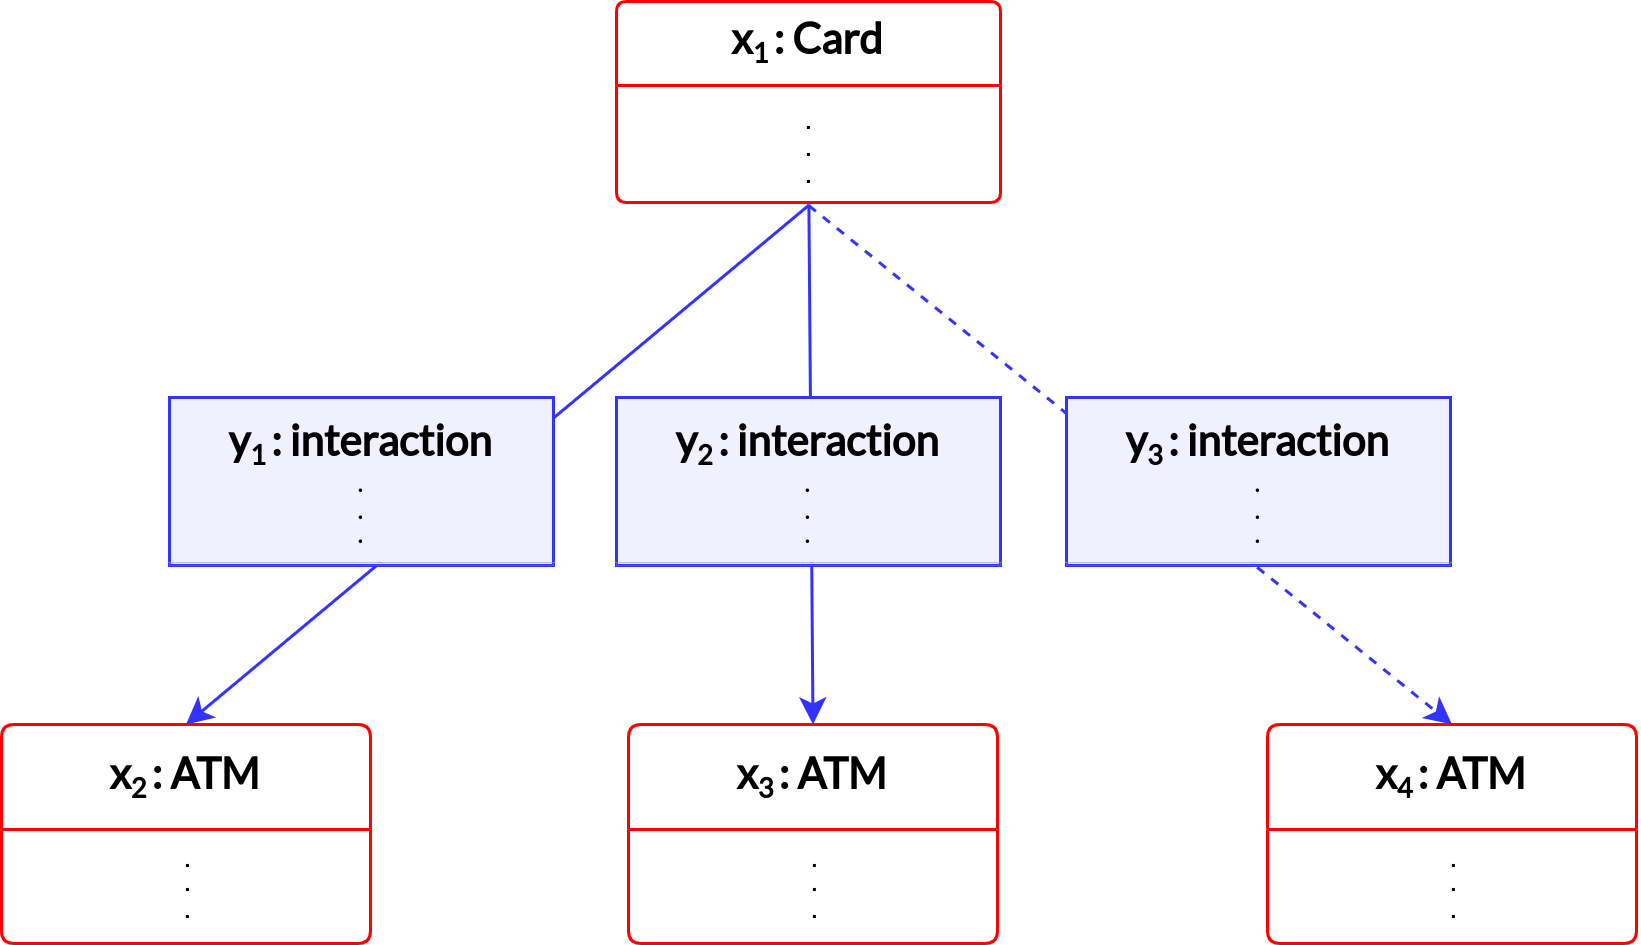
\includegraphics[scale = 0.7]{images/2-QueryModel/fp-I-demo-1.png}
  \caption{Example of a \texttt{Card} $\mathsf{c}$ subgraph $\mathsf{S_c}$ of the volatile property graph. $\mathsf{S_c}$ is an individual node \texttt{Card} $\mathsf{c}$ subgraph of our volatile property graph. It stores all the card-ATM interactions $\mathsf{e_c}$ that are made with \texttt{Card} $\mathsf{c}$ for a considered time interval. The interactions are stored sorted by time.}
  \label{img:fp-I-demo}
\end{figure}

Note that, given the above description, we can either have that:
\begin{itemize}
    \item $\mathsf{F_I(y_2,y_3)}$. Then, we emit an alert of this anomalous scenario produced between the pair $\mathsf{(y_2,y_3)}$. We could continue checking for anomalous scenarios between $\mathsf{y_3}$ and previous edges of the subgraph. However, what we consider important for the bank system is to detect the occurrence of an anomalous scenario in a certain card. Therefore, we consider that, to achieve this, it is enough to emit a single alert of anomalous scenario on this card, and not many related with the same incoming transaction of the same card.
    \item $\neg \mathsf{F_I(y_2,y_3)}$. In this case we analyze whether it would be interesting or not to continue the checking with previous edges of the subgraph, based on assumptions on the fraud checking between previous edges. In particular we can have two cases:
    \begin{itemize}
        \item $\mathsf{F_I(y_1,y_2)}$. Having this it can happen that either $\mathsf{F_I(y_1,y_3)}$ or $\neg \mathsf{F_I(y_1,y_3)}$. In the case of $\mathsf{F_I(y_1,y_3)}$, since $\neg \mathsf{F_I(y_2,y_3)}$, we can infer that the anomalous scenario detected between $\mathsf{y_1}$ and $\mathsf{y_3}$ is a continuation of the same previous anomalous scenario detected between $\mathsf{y_1}$ and $\mathsf{y_2}$. Therefore, we can conclude that this does not constitute a new anomalous scenario that would require an alert.
        \item $\neg \mathsf{F_I(y_1,y_2)}$. It can be shown that \emph{by transitivity}, having \\
        $\neg \mathsf{F_I(y_1,y_2)} \land \neg \mathsf{F_I(y_2,y_3)}
        \implies \neg \mathsf{F_I(y_1,y_3)}$. \\
    \end{itemize}
\end{itemize}

Therefore, we have seen that, it is enough to perform the checking between the pair formed by $\mathsf{e_{new}}$ and the most recent edge of the subgraph $\mathsf{e_{last}}$. $\square$\\


So, we can state that, in an implementation of the detection of the fraud pattern I, for a subgraph $\mathsf{S_c}$, it would be sufficient to only store the last incoming transaction edge $\mathsf{e_{last}}$.\\

Finally, note that due to this algorithmic method, a fraud pattern I alert could be triggered both when an anomalous interaction arrives, $\mathsf{e_{anom}}$, with respect to its previous transaction $\mathsf{e_{prev}}$, emitting the alert pair $\mathsf{(e_{prev}, e_{anom})}$; and also when the subsequent transaction $\mathsf{e_{next}}$ arrives, with respect to the anomalous, emitting the alert pair $\mathsf{(e_{anom}, e_{next})}$.
